\section{Redesigning the wordcount database}
In section \ref{InitialDesign} we established that the design would lead to duplicate or redundant data in the wordcount database.
Namely, the terms occurring in the Term entity set (see section \ref{newdatabaseER}) will not be unique. 
Thus, the database can contain duplicate values.
 
To address this issue, we will create relations using the relational model (see section \ref{relational_databases}) and ensure they are well-designed.
After ensuring that a normal form is reached, we will create the relations using SQL as a DDL.
We will also need to adjust the data access models (see section \ref{models}) to ensure access using EF core.
When implementing the new database structures, we need to ensure that the pipeline is operational and have a minimum downtime. 
Therefore, we have to ensure we can always roll back changes to the code and database structures.
As described in section \ref{CI/CD}, we can easily deploy versions of our code.
By reverting the changes to the old implementation of the models, we can ensure a quick response, should the new implementation fail.
We need to ensure that this is also the case for the database structures.
This is done by taking a dump (backup) of the database, and verifying that no database relations are deleted during the data migration.

\subsection{Redesigning the database model}\label{databaseModelRedesignNF}
We will now create relations describing the new models for the database.
Other groups of the \knox{} pipeline have requested that entities representing articles have a unique Id field, regardless of what is considered good database design.
Similarly, they want a field denoting the total words appearing in the article.

\begin{equation}\label{eq:newDatabaseRelationalModel}
    \begin{split}
        article(\underline{article\_id: \mathbb{Z^+}} title:text,\\ totalwords:\mathbb{Z^+}, publisher\_name \rightarrow publisher), \\
        word(\underline{text:text}),\\
        publisher(\underline{publisher\_name:text}),\\
        occursIn(\underline{text \rightarrow word}, \underline{article\_id \rightarrow article}, count:\mathbb{Z^+})\\
    \end{split}
\end{equation}


Having established these constraints, design have been created using the relational model (equation \ref{eq:newDatabaseRelationalModel}) and the E-R model (figure \ref{fig:newdatabaseRedesignER}).

\begin{figure}[H]
    \centering
    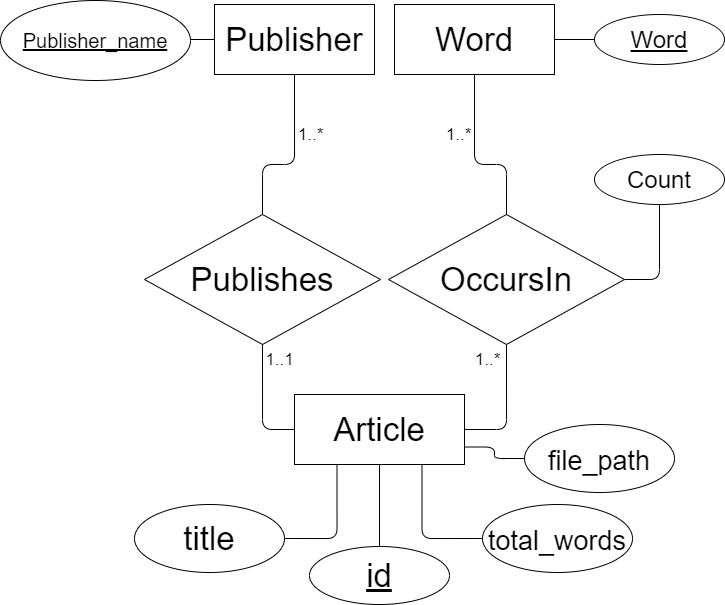
\includegraphics[scale=0.35]{Images/new ER.drawio.png}
    \caption{ER diagram depicting the new model of the database. Notice that the relationship set \textit{Publishes} is not implemented.}
    \label{fig:newdatabaseRedesignER}
\end{figure}
\subsubsection*{Quality of the new design}
Having established the structure of the new database schemas, we can now examine whether they live up to TNF or BCNF (see section \ref{relational_databases}).
This is done by examining the functional dependencies of the relations seen in equation \ref{eq:newDatabaseRelationalModel}.

The \textit{occursIn} relation is in BCNF. 
This is verified when examining the functional dependency of its composite primary key:
\begin{equation*}
 \{text,article\_id\}\rightarrow \{count\}   
\end{equation*}

A unique article cannot identify the text and number of times the text occurs in the article.
Similarly, the number of times the text occurs in the article and the article\_id cannot identify the text of the word.

The \textit{article} relation is in BCNF. 
This is seen when considering the functional dependency of its single, primary key:
\begin{equation*}
    \{article\_id\} \rightarrow \{title, publisher\_name,total\_words\, file\_path\}
\end{equation*}

One could consider using only \textit{title} as key. 
However, some article titles could occur multiple times; this is realized when considering the domain area of the \knox{} search engine\footnote{For instance, the title "The first snow of the season" could be a occurring every year for the same publisher.}. Thus, the composite, primary key $\{ publisher,article\_title \}$ would not guaranteee uniqueness.
One should notice that each of the files in the search engine (represented by the $file\_path$ attribute) can contain multiple articles\footnote{An example of a $file\_path$ could be a path to a newspaper in PDF format, containing many articles about the weather.}.
Thus, the $file\_path$ attribute cannot uniquely identify articles.
Similarly, a PDF file might have chapters (articles) with the same name. For instance, "Review" or "Retrospective".
Thus, using a composite key of \textit{article\_id, file\_path} is not viable. 

The \textit{word} and the \textit{publisher} relations are in BCNF trivially:
\begin{equation*}
    \{ text\} \rightarrow \{text\} \textit{\ and\ } \{ publisher\_name \} \rightarrow \{ publisher\_name\}
\end{equation*}


\subsubsection*{Implementing the models}

Having established the quality of the design of the database structures, we will now how they are implemented. 
Since the relation representing a publisher has not been changed, we will not implement any new designs to it. 
When creating the new tables, we ensure that no loss of data occurs, simply by not dropping the old tables, and renaming them instead. 
The tables can then be dropped later after the full implementations of the new design have been performed.
The renaming of the tables can be seen in Code Snippet \ref{lst:RenamingOldModelsSQL}.

\begin{lstlisting}[
    label=lst:RenamingOldModelsSQL,
    language=SQL,
    caption=SQL script renaming the existing database structures,
    showspaces=false,
    numbers=left,
    numberstyle=\tiny,
    commentstyle=\color{gray},
    escapechar=|
 ]
 ALTER TABLE "Article"
    RENAME TO "Article_Redundant";
ALTER TABLE "Term"
    RENAME TO "Term_Redundant";
\end{lstlisting}

When implementing the new tables, we base them on the just-renamed tables from the old database design.
By doing this, we ensure that all data from the old tables are correctly transferred to the new ones since each of the commands is a transaction. (see section \ref{relational_databases}).
After all data have been transferred to a new table, constraints, foreign- and primary keys are added to the tables. 
This is seen on Code Snippet \ref{lst:CreatingTheNewDBModelsSQL}.
We have ensured that the changes are reversible by creating a script dropping the new tables, and restoring the structure of the old tables.
The script is found in Appendix \ref{SQLBackupScript}.

\begin{lstlisting}[
    label=lst:CreatingTheNewDBModelsSQL,
    language=SQL,
    caption=SQL script creating the tables described in \ref{databaseModelRedesignNF}. Foreign- and primary key constraints are also defined.,
    showspaces=false,
    numbers=left,
    numberstyle=\tiny,
    commentstyle=\color{gray},
    escapechar=|
 ]
CREATE TABLE "Article" AS
SELECT * FROM "Article_Redundant";
ALTER TABLE "Article"
    ADD CONSTRAINT "Id_PRMK" PRIMARY KEY ("Id"),
    ADD FOREIGN KEY ("PublisherName") REFERENCES "Publisher"("PublisherName");

CREATE TABLE "Word" AS
SELECT DISTINCT t."Word" AS "Text" FROM "Term_Redundant" t;
ALTER TABLE "Word" ADD CONSTRAINT "Literal_PRMK" PRIMARY KEY ("Text");

CREATE TABLE "OccursIn" AS
    (
        SELECT "art"."Id" as "ArticleId", "t"."Count",  t."Word"
        FROM"Term_Redundant" t JOIN wordcount.public."Article_Redundant" art ON t."ArticleId" = art."Id"
    );
ALTER TABLE "OccursIn"
    ADD FOREIGN KEY ("ArticleId") REFERENCES "Article"("Id"),
    ADD FOREIGN KEY ("Word") REFERENCES "Word"("Text"),
    ADD PRIMARY KEY ("ArticleId", "Word");
\end{lstlisting}

Having implemented the new database structures, we can redefine the WordRatio view.
Notice that the view is an abstraction over a \texttt{SELECT} statement, thus it is replaceable without loss of data.


\begin{lstlisting}[
    label=lst:DefiningNewView,
    language=SQL,
    caption=SQL script defining a new WordRatio view.,
    showspaces=false,
    numbers=left,
    numberstyle=\tiny,
    commentstyle=\color{gray},
    escapechar=|
 ]
CREATE OR REPLACE view "WordRatio"("ArticleId", "Word", "Count", "Title", "FilePath", "TotalWords", "PublisherName", "Percent") as
SELECT "OccursIn"."ArticleId",
       "OccursIn"."Word",
       "OccursIn"."Count",
       "Article"."Title",
       "Article"."FilePath",
       "Article"."TotalWords",
       "Article"."PublisherName",
       round("OccursIn"."Count"::numeric / "Article"."TotalWords"::numeric * 100::numeric, 2) AS "Percent"
FROM "Article"
         JOIN "OccursIn" ON "OccursIn"."ArticleId" = "Article"."Id"
         JOIN "Publisher" ON "Article"."PublisherName" = "Publisher"."PublisherName";
\end{lstlisting}

\subsection{Result}
Having implemented the new database structure, we can assess the changes to the database. 
The number of words stored in the old \texttt{Term} relation was almost 6,900,000.
The number of words in the just implemented \texttt{Word} relation is 260,000.

